
%\graficarPDF{graf_ej4}{Estimación de la trayectoria.}{fig:ej4}

\begin{figure}[H]
\centering
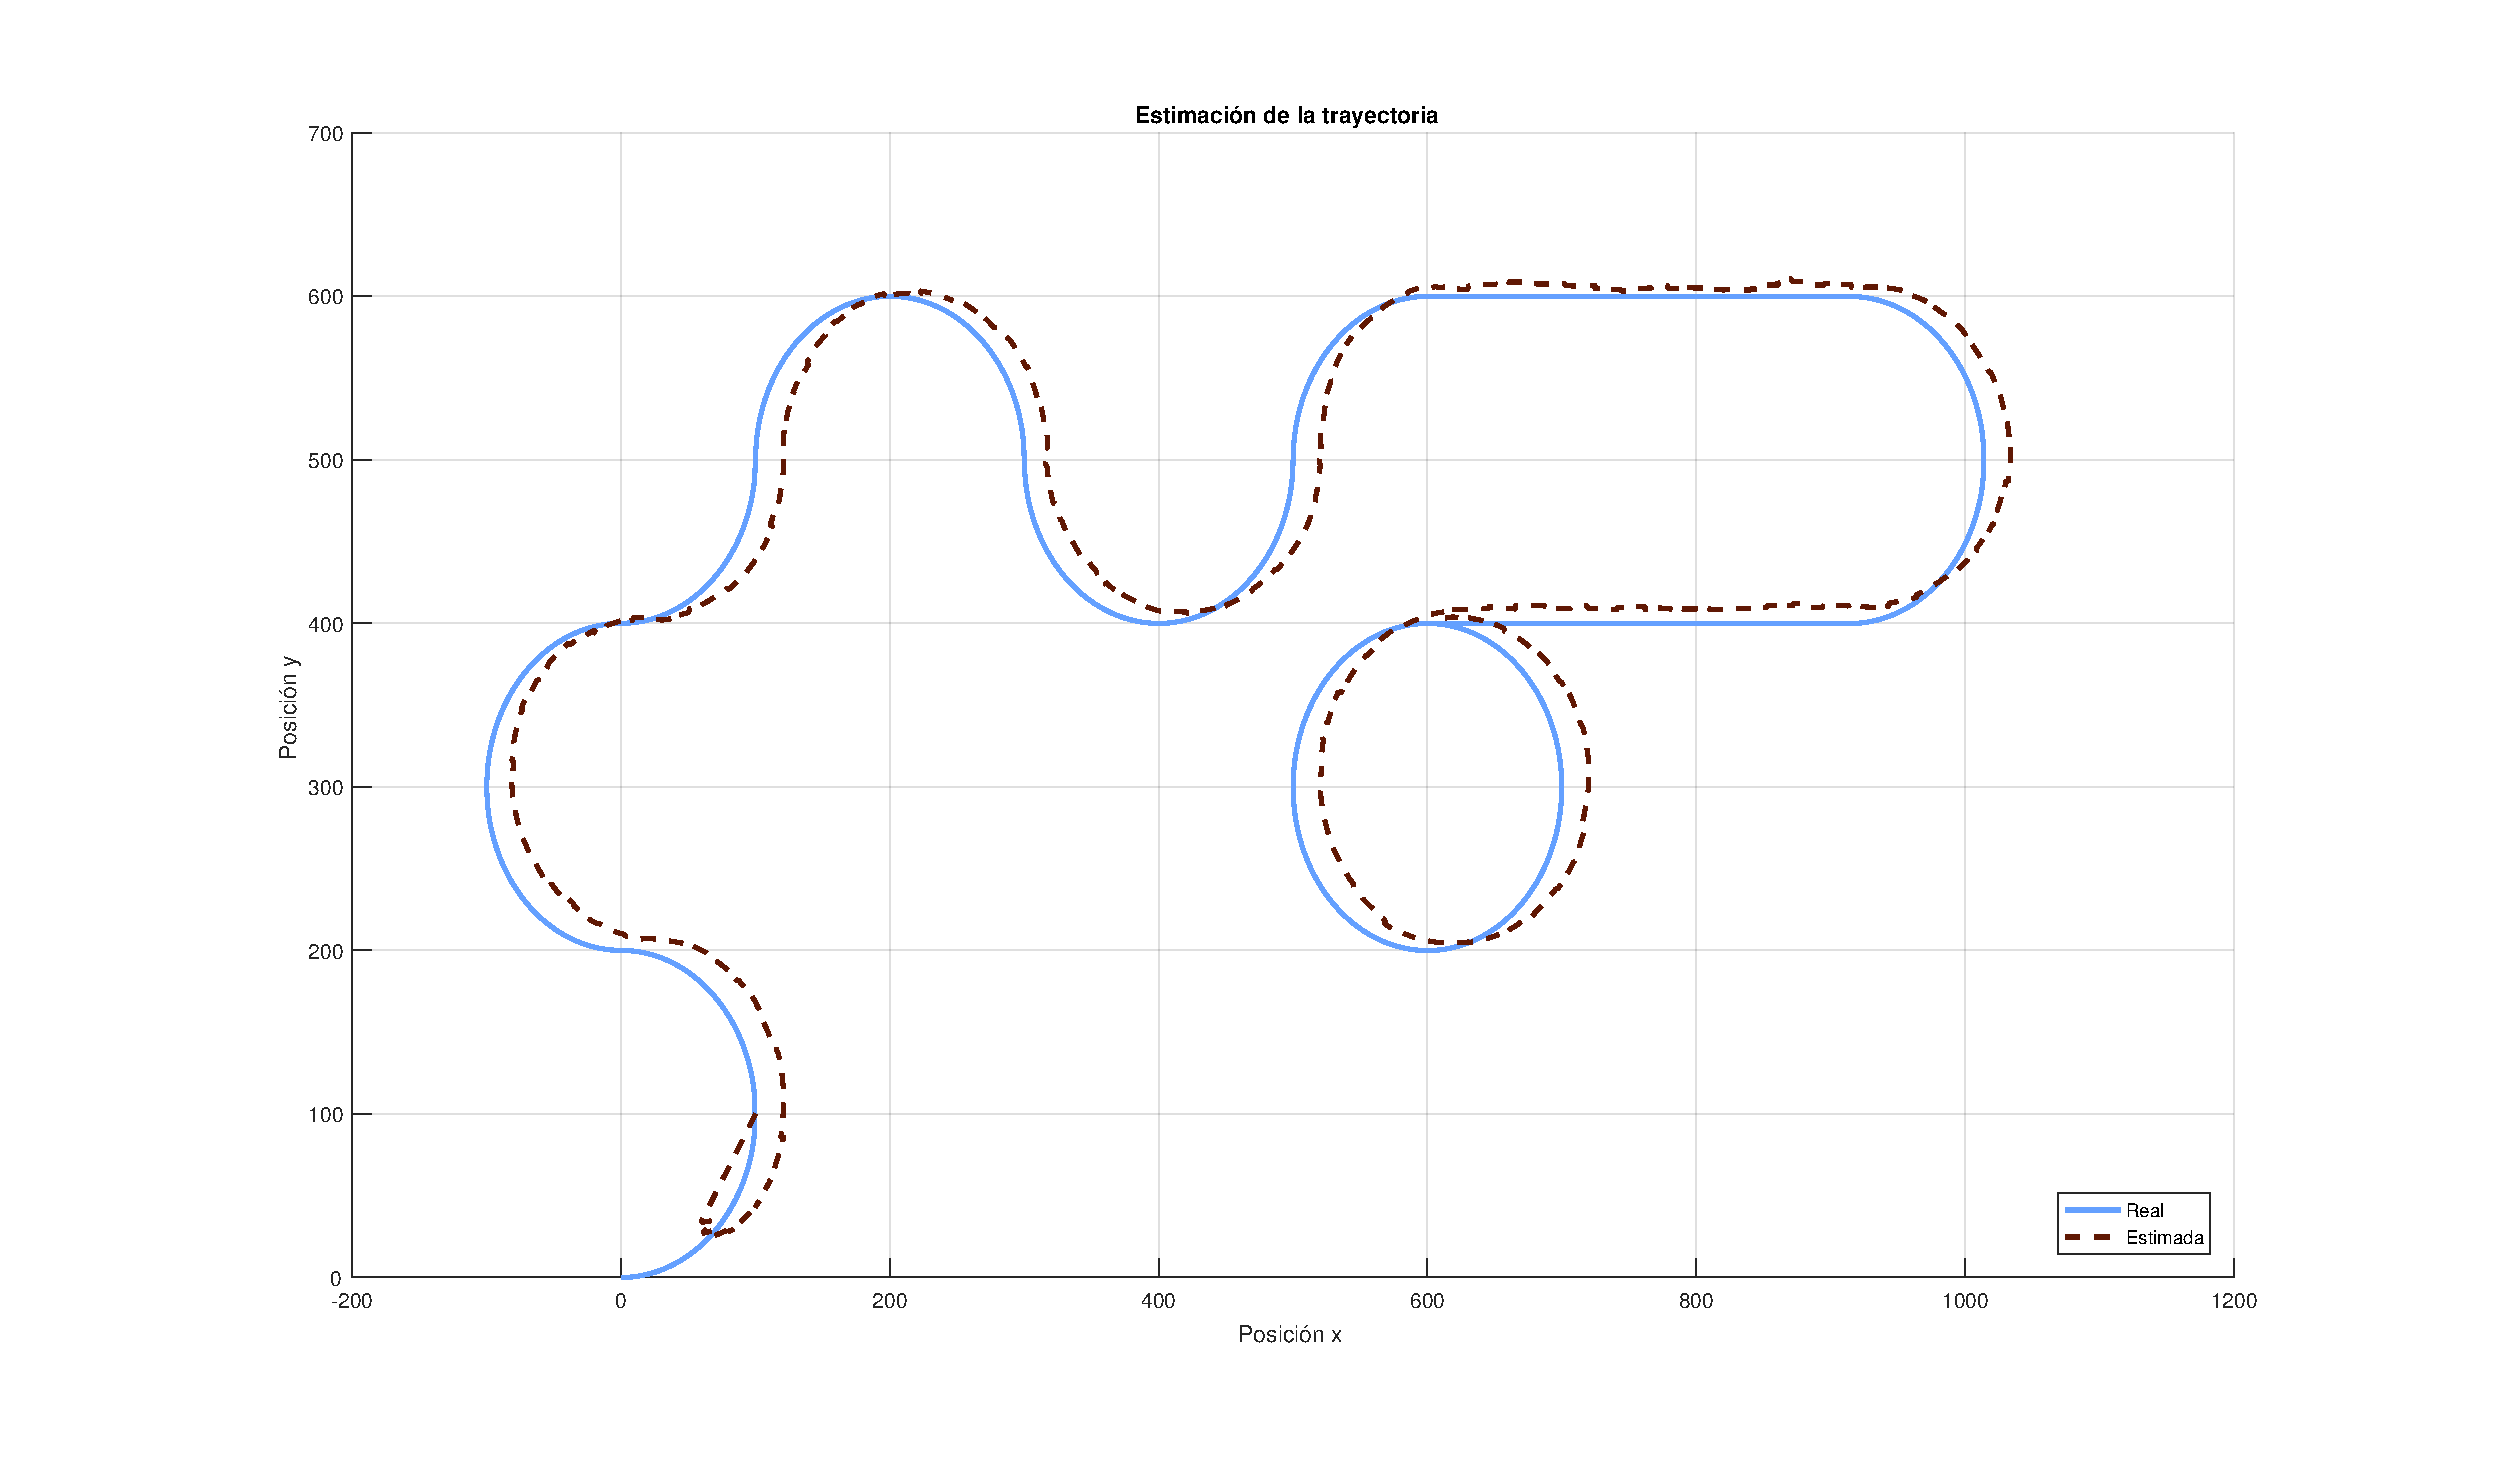
\includegraphics[width=0.9\textwidth,trim= 2cm 2cm 2cm 2cm]{graf_ej4.pdf}
\caption{Estimación de la trayectoria.}
\label{fig:ej4} 
\end{figure}


	El procedimiento para realizar la estimación con sesgo en posición es similar al punto anterior, a excepción de la matriz $C$ donde la identidad se encuentra ahora en las primeras 2 filas de las últimas 2 columnas. Como era de esperar por los resultados obtenidos en el trabajo anterior, no es posible la estimación de la trayectoria dado que los estados del sesgo no son observables. Es por tanto que se obtiene la estimación de la Figura \ref{fig:ej4} que sigue a la trayectoria pero con un \emph{offset} dado por el sesgo que no pudo ser estimado. Ésto se puede ver en el error en posición en la Figura \ref{fig:4pos}, siendo el mismo patrón que en el ejercicio \ref{sec:ej2} pero desplazado verticalmente.

%\graficarPDF{graf_ej4_covinn}{Innovaciones de las poisciones y velocidades en $x^e$ e $y^e$.}{fig:4covinn}

\begin{figure}[H]
\centering
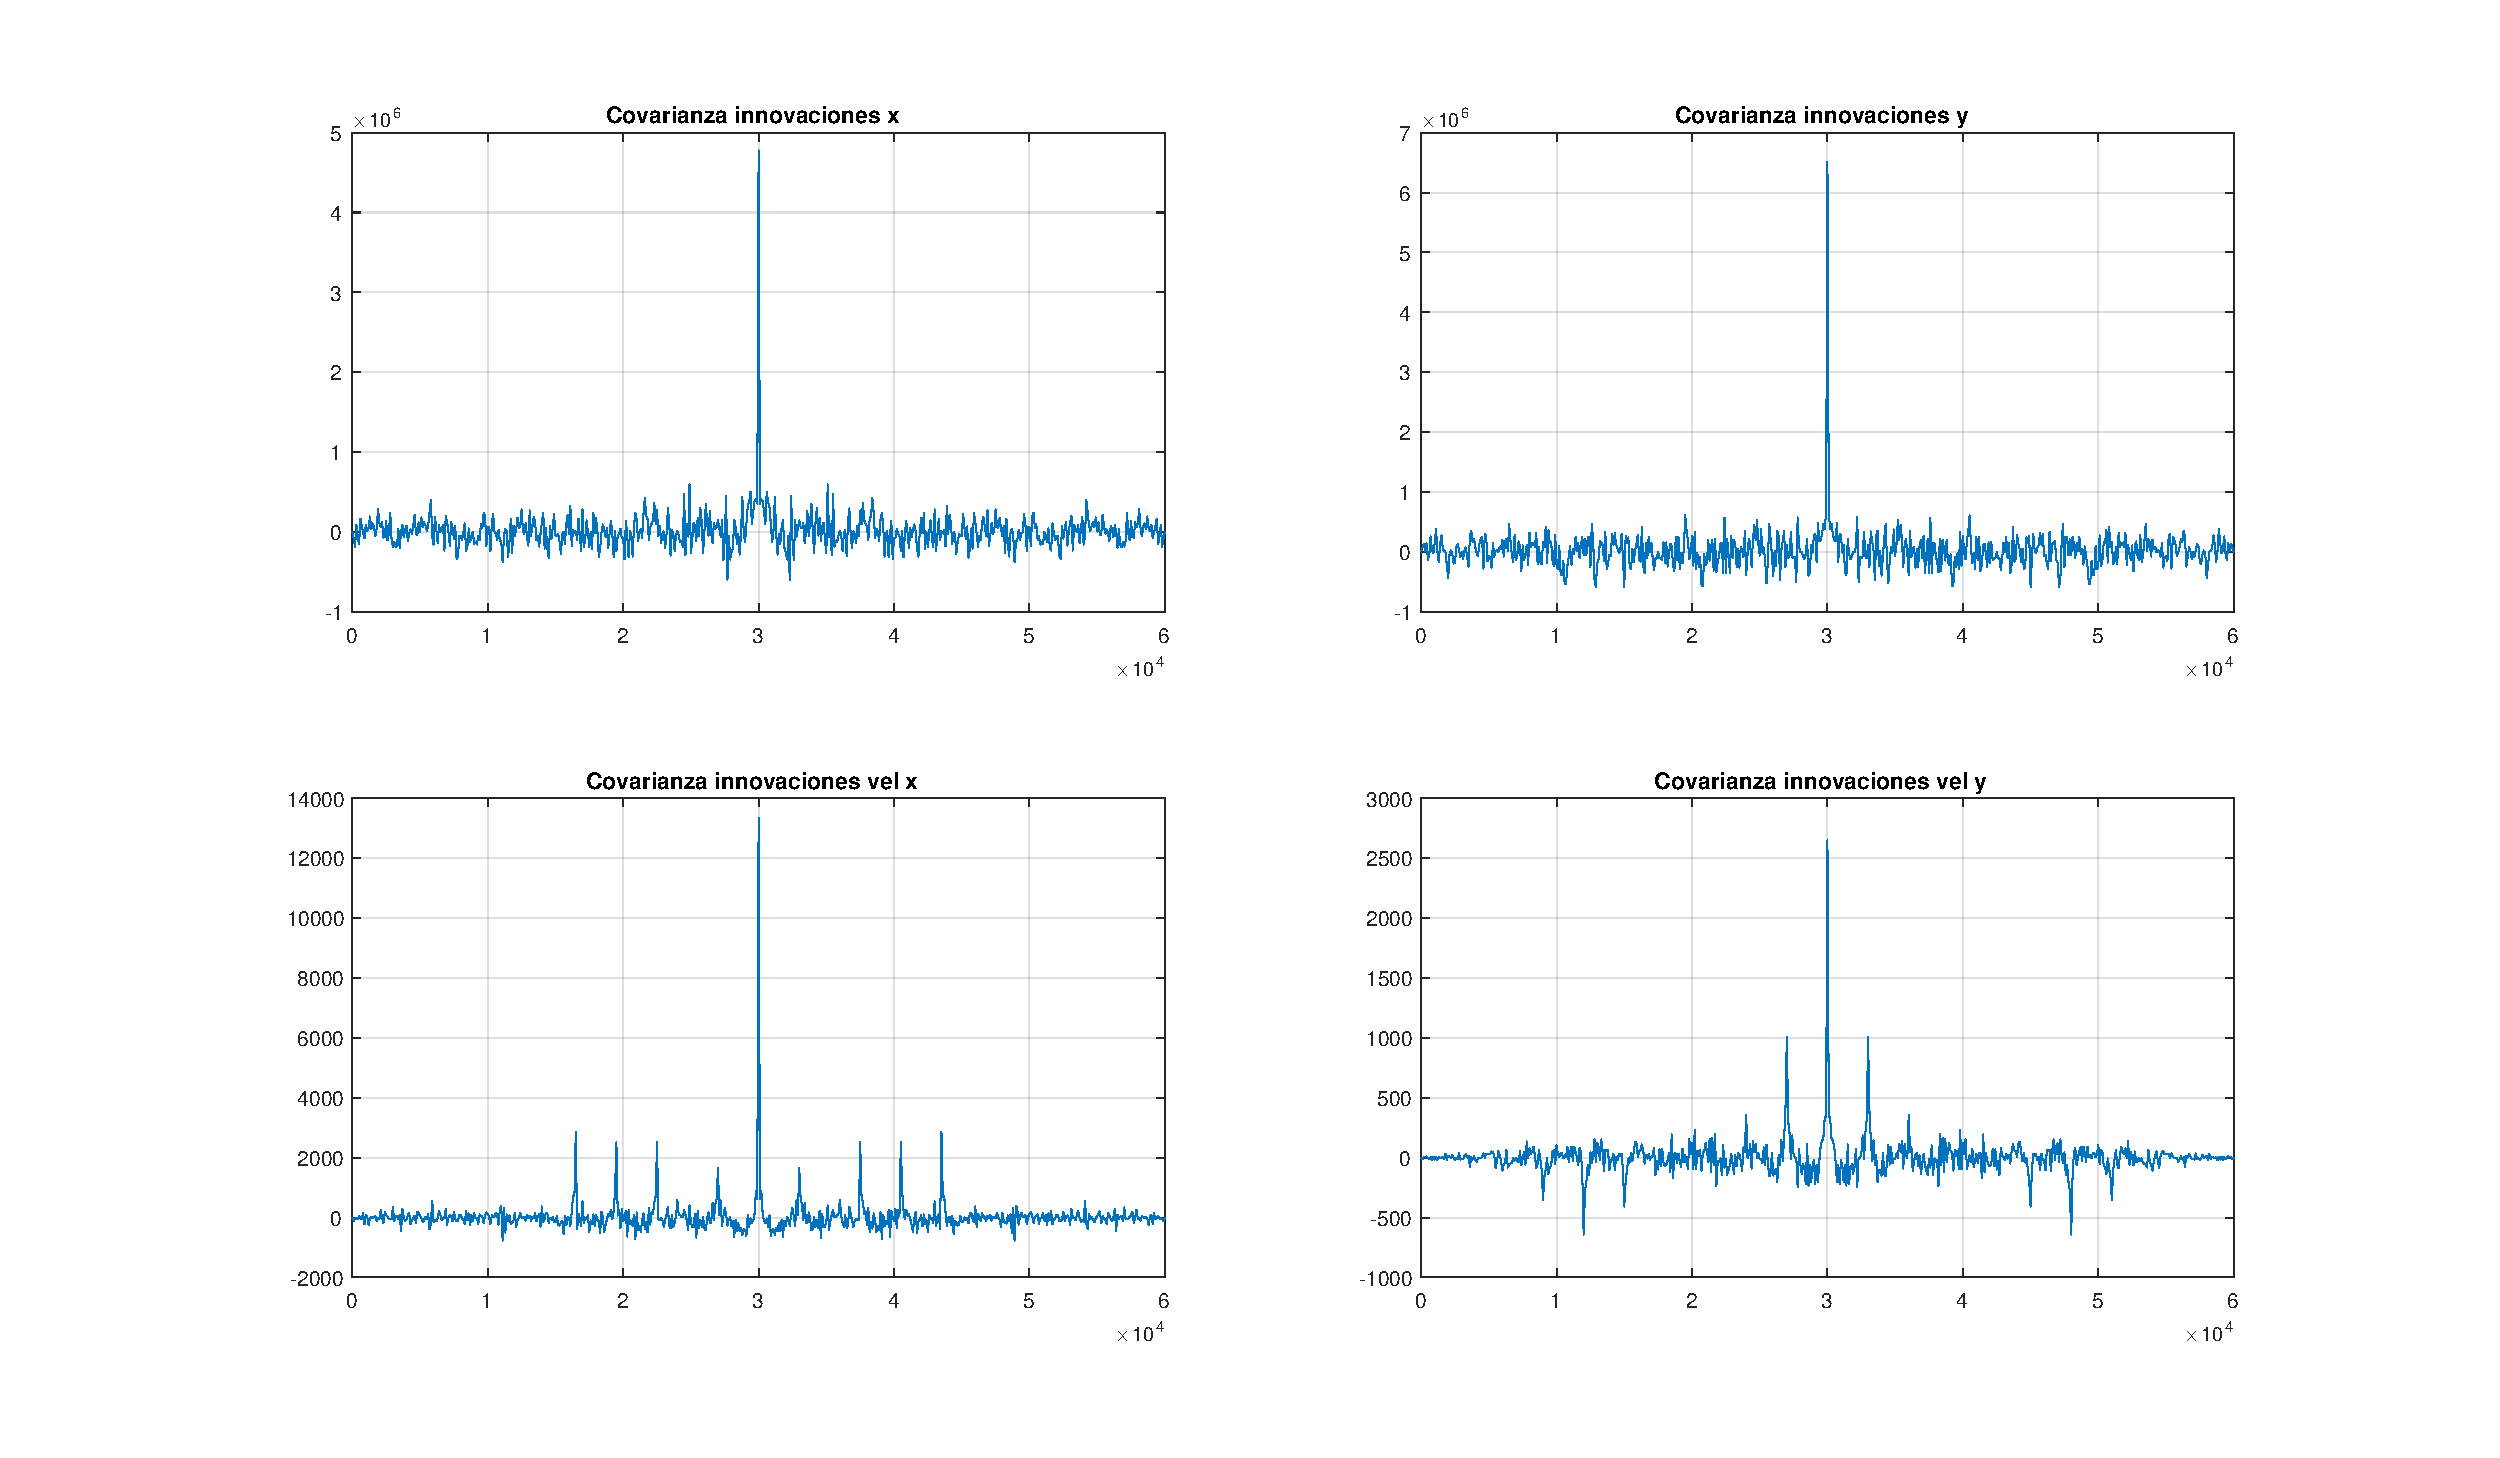
\includegraphics[width=0.9\textwidth, trim=1.5cm 1.5cm 1.5cm 1.5cm]{graf_ej4_covinn.pdf}
\caption{Innovaciones de las posiciones y velocidades en $x^e$ e $y^e$.}
\label{fig:4covinn} 
\end{figure}


\pagebreak

%\graficarPDFa{0 10cm 0 10cm}{graf_ej4_pos}{Posición ej4}{fig:4pos}

\vspace*{\fill}
\begin{figure}[H]
\centering
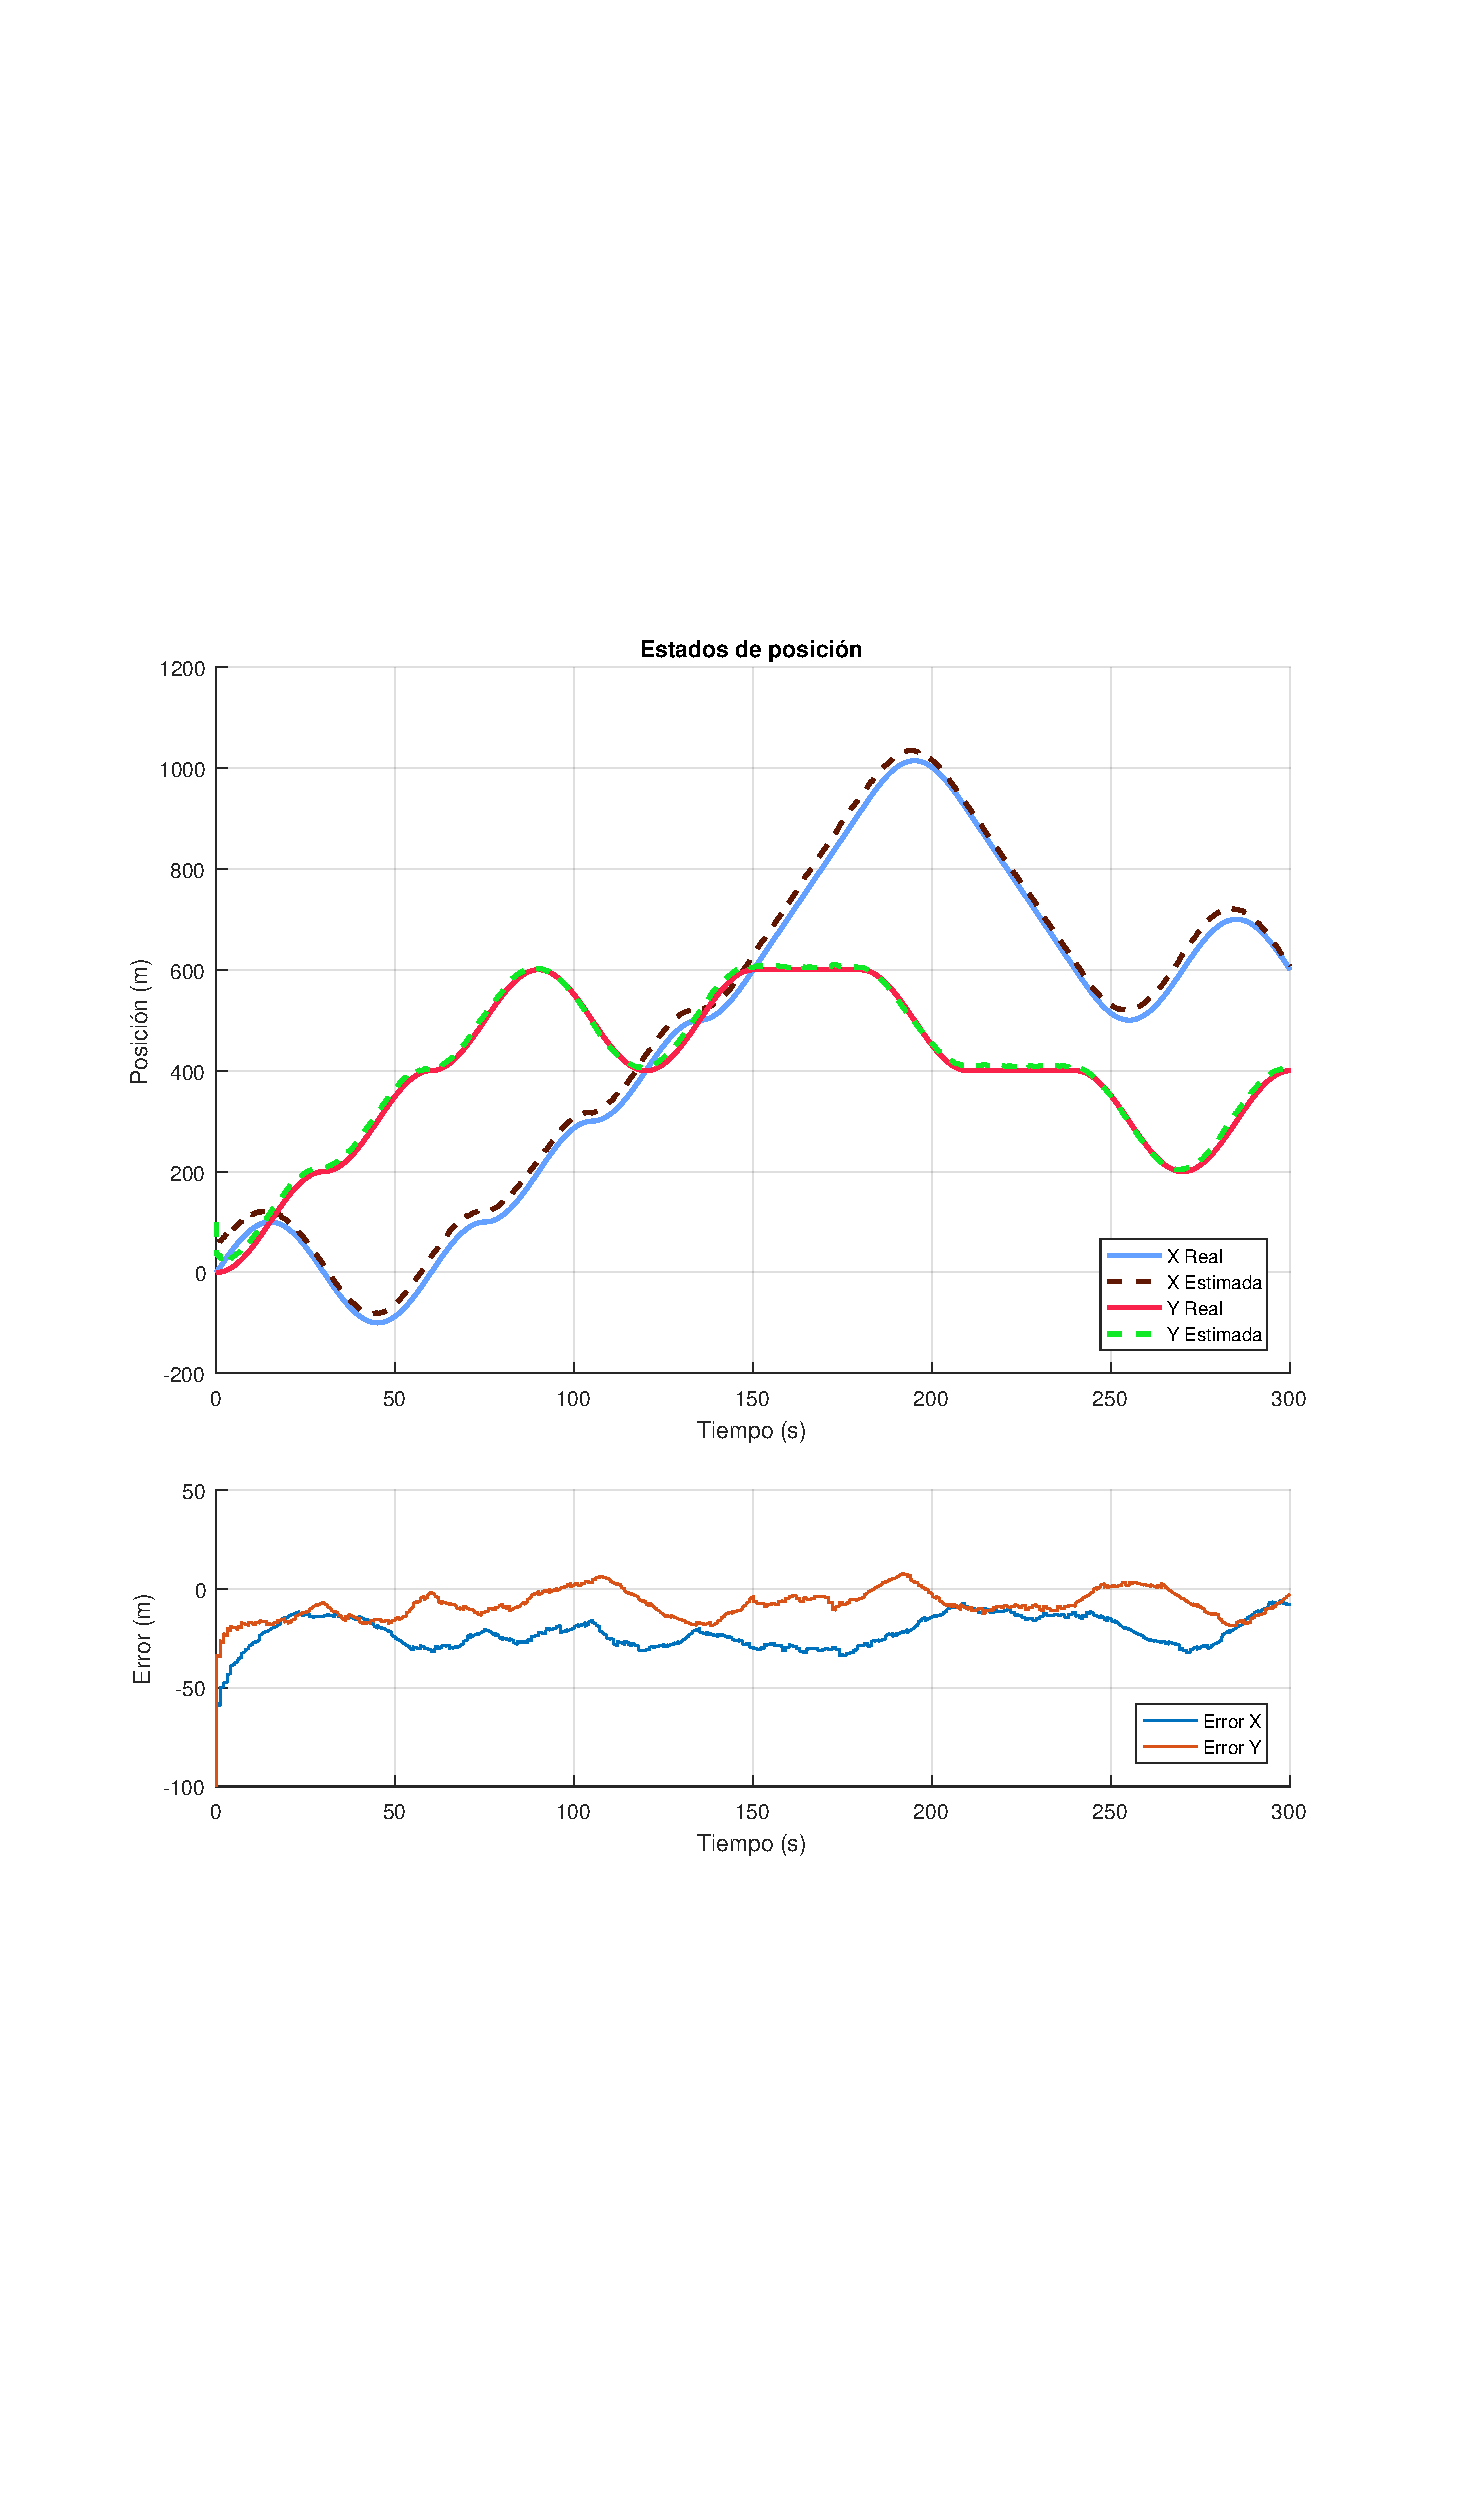
\includegraphics[scale=0.65, trim= 6cm 6cm 6cm 6cm]{graf_ej4_pos.pdf}
\caption{Posición y error en función del tiempo.}
\label{fig:4pos} 
\end{figure}
\vspace*{\fill}

\pagebreak

%\graficarPDFa{0 10cm 0 10cm}{graf_ej4_vel}{Velocidad real y estimada en función del tiempo.}{fig:4vel}

\vspace*{\fill}
\begin{figure}[H]
\centering
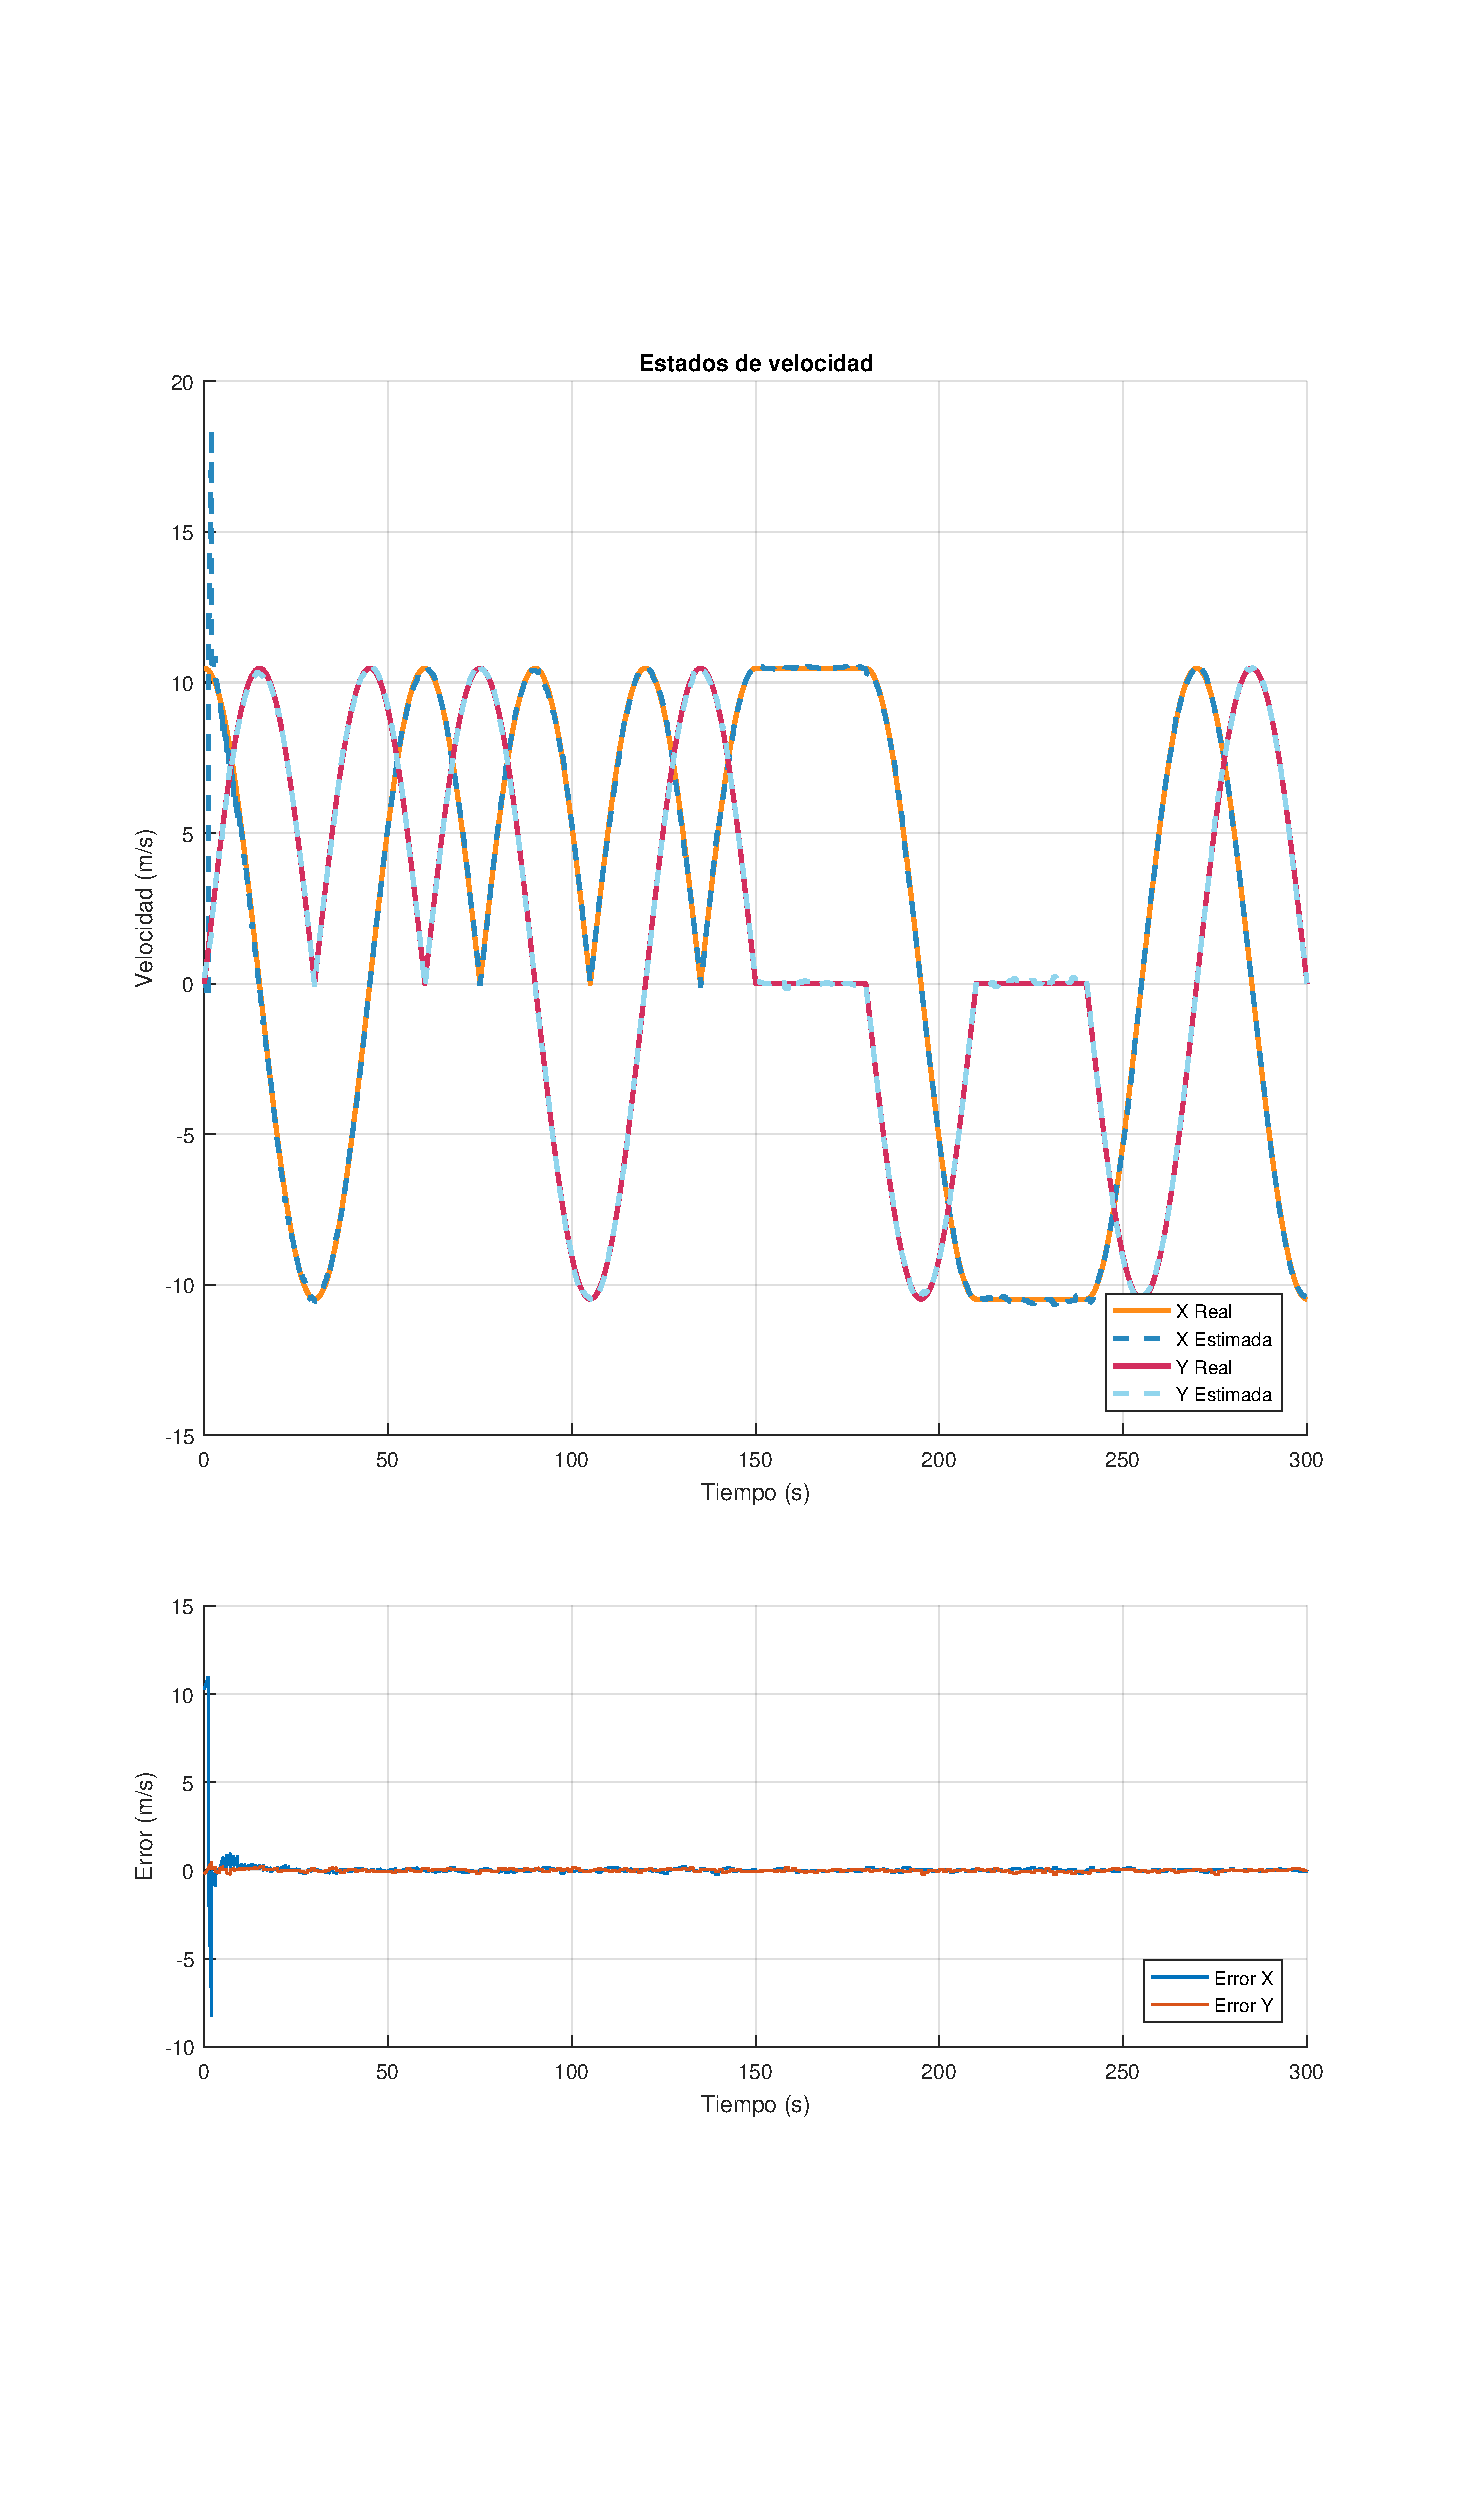
\includegraphics[scale=0.65, trim= 6cm 6cm 6cm 6cm]{graf_ej4_vel.pdf}
\caption{Velocidad real y estimada en función del tiempo.}
\label{fig:4vel} 
\end{figure}
\vspace*{\fill}


\pagebreak
\graficarPDF{graf_ej4_theta}{Valores de los coeficientes de $C^e_b$ en el tiempo.}{fig:4theta}

